\documentclass[12pt,a4paper]{article}
\usepackage[T2A]{fontenc}
\usepackage[utf8]{inputenc}
\usepackage[russian]{babel}
\usepackage{amsmath}
\usepackage{amssymb}
\usepackage{graphicx}
\usepackage{floatrow}
\usepackage{booktabs}
\usepackage{wrapfig}
\usepackage{lipsum}
\usepackage{subcaption}
\usepackage{fancyhdr}

\newcommand{\figref}[1]{(См. рис. \ref{#1})}
\newcommand{\secref}[1]{(См. раздел. \ref{#1})}

\newcommand{\e}[1]{\text{$\cdot10^{#1}$}}

\pagestyle{fancy}
\fancyhead{}
\fancyhead[L]{Работа 3.4.5}
\fancyhead[R]{}
\fancyfoot[C]{\thepage}

\author{\normalsize Выполнил: Голубович Тимур, группа Б01-108 \\
	\normalsize 10.09.2022}
\date{}

\usepackage{float}
\restylefloat{table}
\title{
	\large Отчет о выполнении лабораторной работы 3.4.5 \\
	\Large Петля гистерезиса (динамический метод) \\ 
	
}


\begin{document}
	\maketitle
	
\section*{Цель работы}
Изучение петель гистерезиса различных ферромагнитных материалов в переменных полях.

\section*{Оборудование и приборы} 
Автотрансформатор;
понижающий трансформатор;
амперметр и вольтметр (мультиметры);
резистор;
делитель напряжения;
интегрирующая цепочка;
электронный осциллогра;
тороидальные образцы с двумя обмотками.
	
	
\section*{Теоретическое введение}

Основные характеристики
ферромагнетиков — их коэрцитивное поле $H_c$, магнитная проницаемость
$\mu$, рассеиваемая в виде тепла при перемагничивании мощность — зависят
от частоты перемагничивающего поля. В данной работе кривые гистерезиса ферромагнитных материалов изучаются в поле частоты $\nu_0 =$ 50 Гц
с помощью электронного осциллографа.

Магнитная индукция $ B $ и напряжённость поля $ H $ в ферромагнитном материале неоднозначно связаны между собой: индукция зависит
не только от напряжённости, но и от предыстории образца. Связь между $ B $ и $ H $ типичного ферромагнетика иллюстрирует рис. $\ref{fig:petlya}$.

\begin{figure}[H]
	\centering
	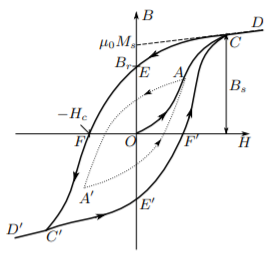
\includegraphics{res/petlya.png}
	\caption{Петля гистерезиса ферромагнетика}
	\label{fig:petlya}
\end{figure}

Если к ферромагнитному образцу прикладывать переменное внешнее
магнитное поле, то его состояние на плоскости $ B-H $ будет изменяться
по замкнутой кривой — петле гистерезиса. Размер петли определяется
максимальным значением напряжённости $ H $ в цикле (например, петля $ AA' $,
обозначенная пунктиром на рис. $\ref{fig:petlya}$). Если амплитуда напряжённости достаточно велика, то образец будет периодически достигать насыщения,
что на рисунке соответствует кривой $ CEFC'E'F'C $ (предельная петля
гистерезиса). Пересечение предельной петли с вертикальной осью соответствует остаточной индукции $B_r$, пересечение с горизонтальной осью
— коэрцитивному полю $H_c$. Крайние точки петель, соответствующие амплитудным значениям $ H $ (например, точка $ A $ на рис. $\ref{fig:petlya}$), лежат на начальной кривой намагничивания ($ OAC $).

\textbf{Измерение магнитной индукции.} Магнитную индукцию $ B $ удобно
определять с помощью ЭДС, возникающей при изменении магнитного
потока $ \Phi $ в катушке, намотанной на образец. Пусть катушка c $ N $ витками плотно охватывает образец сечением $ S $, и индукция $ B $ в образце
однородна. Тогда

\begin{equation}
|B|=\frac{1}{SN}\int\mathcal{E} dt.
\label{eq:|B|}
\end{equation}

\begin{wrapfigure}{r}{0.35\linewidth}
	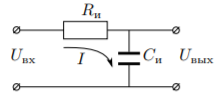
\includegraphics[width=\linewidth]{res/int.png}
	\caption{Интегрирующая ячейка}
	\label{fig:int}
\end{wrapfigure}

Для интегрирования в работе используется интегрирующая $ RC $-цепочка (рис. $ \ref{fig:int} $).
«Входное» напряжение от источника $U_{\text{вх}}(t)$ подаётся на последовательно соединённые резистор $R_\text{и}$ и конденсатор $C_\text{и}$. <<Выходное>>
напряжение $U_{\text{вых}}(t)$ снимается с конденсатора. Предположим, что 1) сопротивление источника мало по сравнению с $R_\text{и}$, 2) выходное сопротивление (сопротивление на входе осциллографа), напротив, велико: $R_{\text{вых}}$ $ \gg $ $R_\text{и}$ и, наконец, 3) сопротивление $R_\text{и}$ достаточно велико, так что почти всё падение напряжения приходится на него, а $U_{\text{вых}}$ $\ll$ $U_{\text{вх}}$. В таком случае ток цепи равен I = ($U_{\text{вх}}$ - $U_{\text{вых}}$)/$R_\text{и}$ $\approx$ $U_{\text{вх}}$/$R_\text{и}$, и входное и выходное сопротивление связаны соотношением

\begin{equation}
U_{\text{вых}} = \frac{q}{C_\text{и}} = \frac{1}{C_\text{и}}\int\limits_0^t Idt \approx \frac{1}{\tau_\text{и}} \int\limits_0^t U_{\text{вх}}dt,
\label{eq:U_ext}
\end{equation}

где $\tau_\text{и}=R_\text{и}C_\text{и}$ - постоянная времени $ RC $ - цепочки. Для индукции поля из ($\ref{eq:|B|}$) получаем 

\begin{equation}
|B|=\frac{1}{SN}\int U_{\text{вх}} dt=\frac{\tau_\text{и}}{SN}U_{\text{вых}}.
\label{eq:|B|new}
\end{equation}

\textbf{Замечание.} Уточним критерий применимости соотношения ($\ref{eq:U_ext}$). Пусть на вход интегрирующей ячейки подан синусоидальный сигнал с частотой $\omega_0$. Тогда, пользуясь методом комплексных амплитуд, нетрудно найти отношение амплитуд входного и выходного напряжений:

\begin{equation}
\frac{U_{\text{вых}}}{U_{\text{вх}}}=\frac{1/\omega_0C}{\sqrt{R^2+1/(\omega_0C)^2}}.
\end{equation}

Тогда неравенство $U_{\text{вых}} \ll U_{\text{вх}}$ реализуется, если 

\begin{equation}
\tau \equiv RC\gg \frac{1}{\omega_0}
\end{equation}

(импеданс конденсатора мал по сравнению сопротивлением резистора).
В таком случае для синусоидального сигнала имеем

\begin{equation}
\frac{U_{\text{вых}}}{U_{\text{вх}}}\approx\frac{1}{\omega_0\tau}.
\label{eq:tau}
\end{equation}

В общем случае, если $\omega_0$ — частота самой низкой гармоники в спектре
произвольного входного сигнала, то при $\omega_0\tau \gg 1$ неравенство $U_{\text{вых}} \ll U_{\text{вх}}$ выполняется на любой частоте $\omega > \omega_0$.

Рассчитать дифференциальную магнитную проницаемость можно по формуле:

\begin{equation}
    \mu_\text{диф}=\frac{dB}{dH}=\frac{B_\text{дел}}{H_\text{дел}}\cdot \frac{dy}{dx}
\end{equation}



\section*{Экспериментальная установка}

Схема установки изображена на рис. $\ref{fig:scheme}$. Напряжение сети (220 В,
50 Гц) с помощью трансформаторного блока Т, состоящего из регулировочного автотрансформатора и разделительного понижающего трансформатора, подаётся на намагничивающую обмотку $N_0$ исследуемого образца.

\begin{figure}[h]
	\centering
	\caption{ Схема установки для исследования намагничивания образцов}
	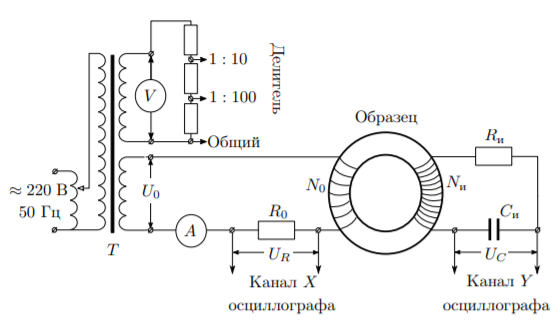
\includegraphics{res/scheme.png}
	\label{fig:scheme}
\end{figure}

В цепь намагничивающей катушки, на которую подаётся некоторое
напряжение $U_0$, последовательно включено сопротивление $R_0$. Напряжение на $R_0$, равное $U_R$= $R_0I_0$, где $I_0$ — ток в намагничивающей обмотке $N_0$, подаётся на канал $ X $ осциллографа. Связь напряжённости $ H $ в
образце и тока $I_0$ рассчитывается по теореме о циркуляции. 
Действующее значение переменного тока в обмотке $N_0$ измеряется амперметром A.
Для измерения магнитной индукции $ B $ с измерительной обмотки $N_\text{и}$
на вход $ RC $-цепочки подаётся напряжение $U_\text{и}$ ($U_{\text{вх}}$), пропорциональное
производной $ dB/dt $. С интегрирующей ёмкости $C_\text{и}$ снимается напряжение $U_C$ ($U_{\text{вых}}$), пропорциональное величине $ B $, и подаётся на вход $ Y $
осциллографа. Значение индукции поля $ B $ рассчитывается по формуле ($\ref{eq:|B|new}$).
Замкнутая кривая, возникающая на экране, воспроизводит в некотором масштабе (различном для осей $ X $ и $ Y $) петлю гистерезиса. Чтобы придать этой кривой количественный смысл, необходимо установить
м

\section*{Ход работы}

\subsection*{Измерение петель гистерезиса}

Соберем схему согласно рис. $\ref{fig:scheme}$. Подберем ток питания в намагничивающей обмотке с помощью автотрансформатора и коэффициенты усиления ЭО таким образом, чтобы предельная петля гистерезиса занимала большую часть экрана. Приведем характерные значения катушек разных материалов в таблице \ref{tab:har_kat}.

\begin{table}[H]
	\caption{Характеристики катушек}
	\begin{tabular}{cccc}
\toprule
& Феррит & Пермаллой & Кремниевое железо \\
\midrule
$N_0$               & 42    & 20    & 25    \\
$N_\text{и}$        & 400   & 300   & 250   \\
$S^2, \text{см}^2$  & 3,00  & 0,76  & 2,00  \\
$2\pi R$, см        & 25,0  & 13,3  & 11,0  \\
\bottomrule
\end{tabular}
	\label{tab:har_kat}
\end{table}


Для каждого образца получим передельные петли гистерезиса, по коэффициентам усиления ЭО $K_x$ и $K_y$ рассчитаем масштабы, определим двойные амплитуды коэрцетивной силы $ 2x(c) $ и индукции насыщения $ 2y(s) $. Масштабы по осям $ X $ и $ Y $ рассчитаем по формулам 
$H=\frac{IN_0}{2\pi R},\ где\ I=\frac{K_x}{R_0};\ B=\frac{R_\text{и}C_\text{и}U_{\text{вых}}}{SN_\text{и}},$ где $U_{\text{вых}}=K_y$. Результаты измерений и вычислений занесём в таблицу \ref{tab:izm}.

\begin{table}[H]
    \caption{Результаты измерений}
    \begin{tabular}{cccc}
\toprule
& Феррит & Пермаллой & Кремниевое железо \\
\midrule
$2x(c)$, дел              & 42    & 20    & 25    \\
$2y(s)$, дел              & 400   & 300   & 250   \\
$K_x$, мВ/дел               & 3,00  & 0,76  & 2,00  \\
$K_y$, мВ/дел               & 25,0  & 13,3  & 11,0  \\
$I_\text{эфф}$, мА          & 363   & 360   & 380   \\
А$\cdot$м$^{-1}/\text{дел}$ & 16,80 & 15,04 & 22,73 \\
$B, \text{Тл}/\text{дел}$   & 0,33  & 1,75  & 0,80  \\
\bottomrule
\end{tabular}

	\label{tab:izm}
\end{table}

Теперь, зная масштабы по осям, можно определить значения коэрцетивной силы $ H_c $
и индукции насыщения $ B_s $. Результаты заносим в таблицу \ref{tab:vichisl}.

\begin{table}[H]
    \caption{Результаты вычислений}
    \begin{tabular}{cccc}
\toprule
& Феррит & Пермаллой & Кремниевое железо \\
\midrule
$H_c$, А/м          & 50    & 60    & 91    \\
$\sigma_{H_c}$, А/м & 6     & 8     & 10    \\
$B_s$, Тл           & 0,90  & 3,9   & 2,0   \\
$\sigma_{B_s}$, Тл  & 0,08  & 0,2   & 0,10  \\
\bottomrule
\end{tabular}

	\label{tab:vichisl}
\end{table}

Также в следующую таблицу \ref{tab:tab} занесём табличные данные для значений коэрцетивной силы $ H_c $ и индукции насыщения $ B_s $.

\begin{table}[H]
    \caption{Табличные данные}
    \begin{tabular}{cccc}
\toprule
& Феррит & Пермаллой & Кремниевое железо \\
\midrule
$H_c$, А/м  & 20    & 11-40 & 50-100    \\
$B_s$, Тл   & 0,27  & 1,51  & 1,21      \\
\bottomrule
\end{tabular}

	\label{tab:tab}
\end{table}

Сравнивая полученные данные с табличными можно утверждать, что они совпадают, по крайней мере по порядку величины. Также приведём фотографии предельных петель гистерезиса.

\begin{figure}[h!]
	\centering
	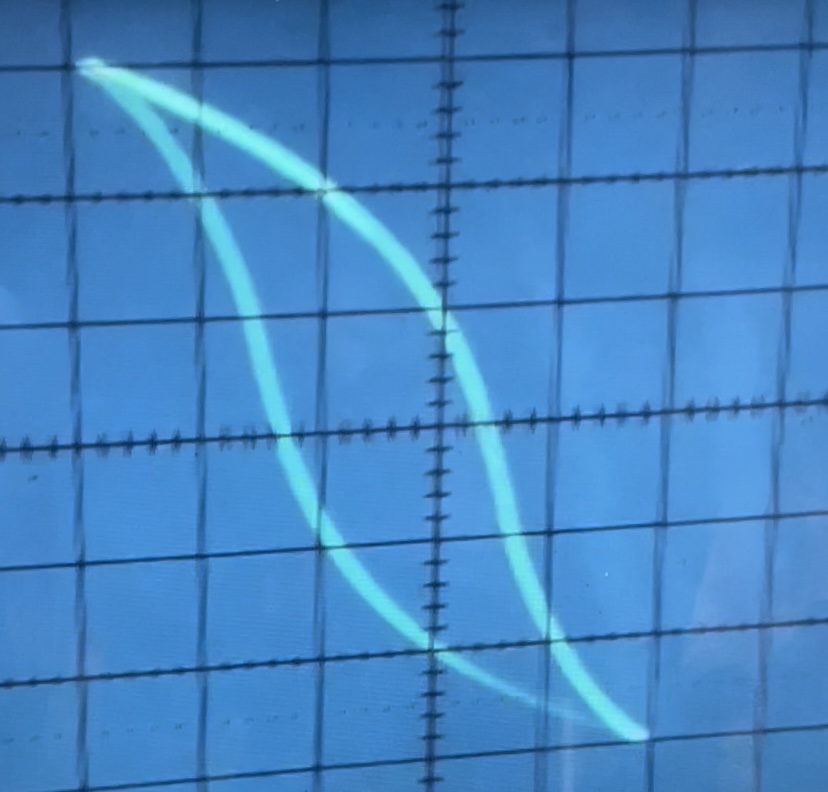
\includegraphics[width=8cm]{src/ferrit.jpg}
	\caption{Предельная петля гистерезиса феррита}
\end{figure}
\begin{figure}[h!]
	\centering
	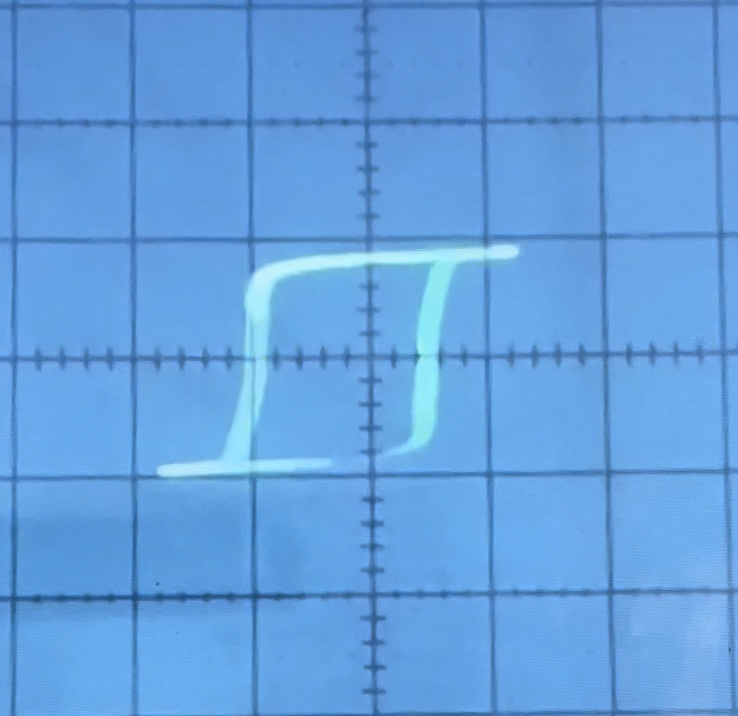
\includegraphics[width=8cm]{src/permal.jpg}
	\caption{Предельная петля гистерезиса пермаллоя}
\end{figure}
\newpage
\begin{figure}[h!]
	\centering
	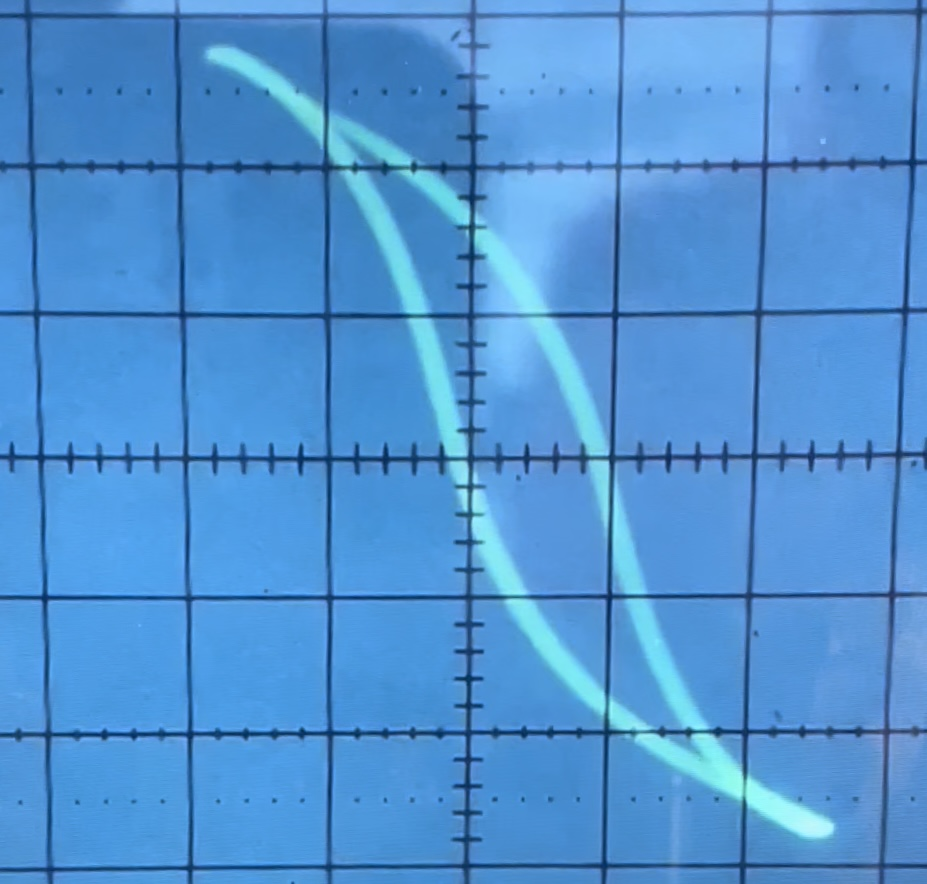
\includegraphics[width=8cm]{src/silicon_fe.jpg}
	\caption{Предельная петля гистерезиса для кремнистого железа}
\end{figure}

\subsection*{Построение начальных кривых намагничивания}

Построим графики начальных кривых намагничивания по таблице \ref{tab:beg}. После этого проведём интерполяцию полиномами и рассчитаем значения начальных и максимальных значений дифференциальной магнитной проницаемости. Соответсвующие значения запишем в таблицу \ref{tab:mu}. 

\begin{table}[H]
    \caption{Начальные кривые намагничивания}
    \begin{table}
\begin{tabular}{ccc|ccc|ccc}
\toprule
\multicolumn{3}{c}{Феррит} & \multicolumn{3}{c}{Кремниевое железо} & \multicolumn{3}{c}{Пермаллой} \\
$I$, А & $X$, дел & $Y$, дел & $I$, А & $X$, дел & $Y$, дел & $I$, А & $X$, дел & $Y$, дел \\
\midrule
357 & 2,7	& 3,0 & 360	& 2,7 & 3,0 & 319 & 3,4	& 1,0   \\
316 & 2,2   & 2,9 & 317 & 2,3 & 2,8 & 288 & 3,0 & 1,0   \\
286 & 2,0   & 2,8 & 284 & 1,9 & 2,6 & 246 & 2,3	& 1,0   \\
247 & 1,8   & 2,6 & 247 & 1,6 & 2,2 & 217 & 2,0 & 1,0   \\
213 & 1,4   & 2,1 & 210 & 1,4 & 2,0 & 184 & 1,4 & 1,0   \\
175 & 1,2   & 1,8 & 182 & 1,2 & 1,6 & 146 & 0,9 & 0,8   \\
147 & 1,0	& 1,4 & 120 & 0,7 &	0,8	& 111 & 0,3	& 0,4   \\
117 & 0,8	& 1,0 & 90  & 0,5 &	0,5	& 50  & 0,2	& 0,2   \\
87  & 0,6	& 0,7 & 57  & 0,3 &	0,2	& 0   & 0   & 0     \\
47  & 0,4	& 0,3 & 28  & 0,2 &	0,1	               		\\
0   & 0     & 0   & 0   & 0   & 0                  		\\	
\bottomrule
\end{tabular}
\end{table}
	\label{tab:beg}
\end{table}

\begin{figure}[h!]
	\centering
	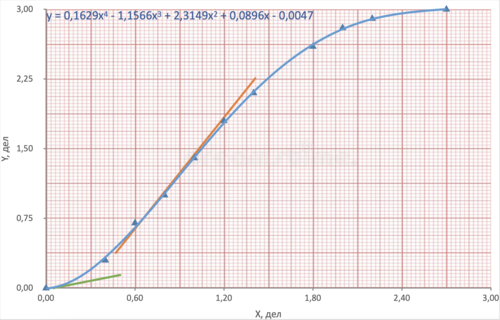
\includegraphics[width = 12 cm]{src/fer.png}
	\caption{Начальная кривая намагничивания феррита}
\end{figure}
\begin{figure}[h!]
	\centering
	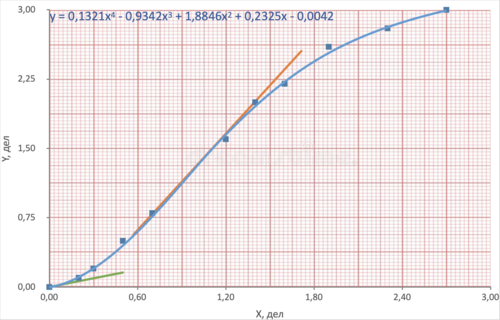
\includegraphics[width = 12 cm]{src/sil.png}
	\caption{Начальная кривая намагничивания кремнистого железа}
\end{figure}
\begin{figure}[h!]
	\centering
	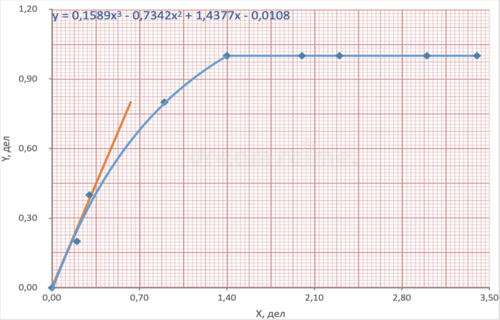
\includegraphics[width = 12 cm]{src/perm.png}
	\caption{Начальная кривая намагничивания пермаллоя}
\end{figure}

\begin{table}[H]
    \caption{Значения дифференциальной магнитной проницаемости}
    \begin{tabular}{cccc}
\toprule
& Феррит & Пермаллой & Кремниевое железо \\
\midrule
$\mu_\text{нач}, 10^{-3}\cdot\text{Тл}\cdot\text{А/м}$ & 6,2    & 27,1  & 44,5    \\
$\mu_\text{max}, 10^{-3}\cdot\text{Тл}\cdot\text{А/м}$ & 39,6   & 203,0 & 44,5    \\
\bottomrule
\end{tabular}

	\label{tab:mu}
\end{table}

\subsection*{Расчёт постоянной времени цепочки}

Рассчитаем постоянную времени по формуле (\ref{eq:tau}) из таблицы \ref{tab:tau}.

$$\tau = \frac{2y\cdot K_y}{\Omega \cdot 2x\cdot K_x } = (0,35 \pm 0,02) \;\;\;\; \varepsilon_{\gamma}=6\%$$

\begin{table}[H]
    \caption{Расчёт постоянной времени цепочки}
    \centering
    \begin{tabular}{cccccccccc}
\toprule
$2x(c)$, дел & $2y(c)$, дел & $K_x$, мВ/дел & $K_y$, В/дел & $U_\text{вх}$, В & $U_\text{вых}$, В & $\tau$, с & $\sigma_{\tau}$, с & $\varepsilon_{\tau}, \%$\\
\midrule
5,4 & 6,0 & 20 & 2,00 & 12,000 & 0,108 & 0,35 & 0,02 & 6 \\
\bottomrule
\end{tabular}

	\label{tab:tau}
\end{table}


Результат довольно хорошо согласуется с теоретическим значением $\tau = 0,4$ с.

\section*{Вывод}

В результате работы были получены результаты для трёх образцов: феррита, кремниевого железа и пермаллоя. Была рассчитана индукция насыщения Bs, коэрцитивное поле Hc, остаточная индукция Br, а также определены начальные и максимальные значения дифференциальной магнитной проницаемости. Измерена постоянная времени данной цепочки.

\newpage
\begin{thebibliography}{9}
	\bibitem{Siv} Сивухин Д. В. \emph{Общий курс физики. Том 3 Электричество и магнетизм}, 2004
	\bibitem{kirich} Кириченко Н.А. \emph{Электричество и магнетизм.}, 2011
	\bibitem{max} \emph{Лабораторный практикум по общей физике. В 3 томах. Том 2. Электричество и магнетизм: учебное пособие} под ред. А. В. Максимычева, М. Г. Никулина
\end{thebibliography}
\end{document}
\end{document}